\documentclass[tikz,border=2pt]{standalone}
\usetikzlibrary{positioning,arrows.meta,fit,backgrounds}
\begin{document}
% ClosetVTON architecture (vector; notation matches Section "Materials and Methods").
% Requires: tikz with libraries positioning, arrows.meta, fit, backgrounds.
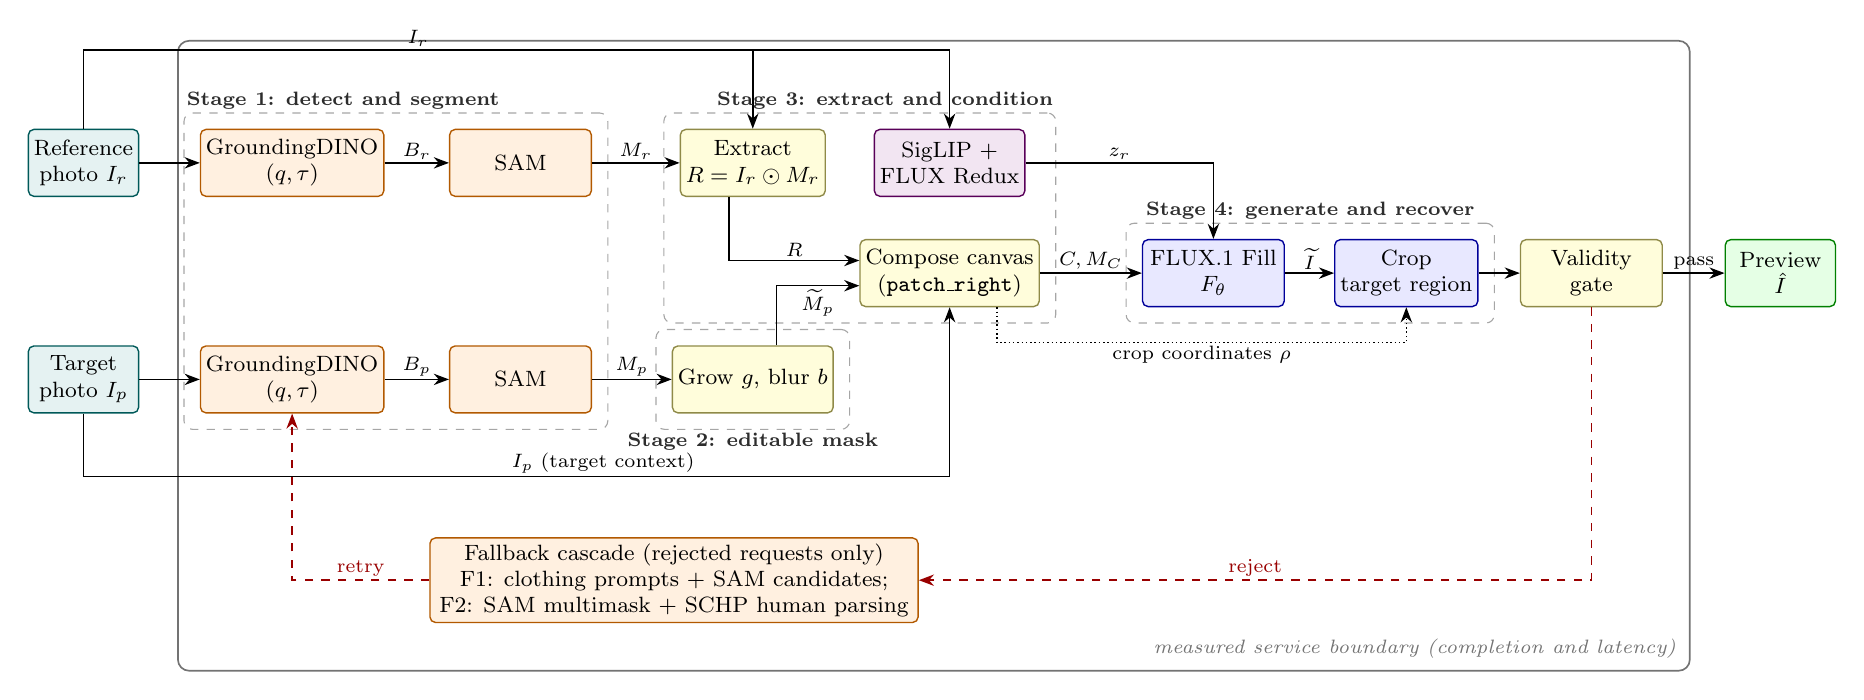
\begin{tikzpicture}[
  font=\footnotesize, >=Stealth,
  box/.style={draw, rounded corners=2pt, align=center, minimum height=8.5mm, minimum width=18mm, inner sep=2pt, line width=0.5pt},
  inbox/.style={box, fill=teal!10, draw=teal!70!black, minimum width=14mm},
  perbox/.style={box, fill=orange!12, draw=orange!70!black},
  prepbox/.style={box, fill=yellow!14, draw=yellow!50!black},
  condbox/.style={box, fill=violet!10, draw=violet!70!black},
  genbox/.style={box, fill=blue!9, draw=blue!60!black},
  outbox/.style={box, fill=green!10, draw=green!50!black, minimum width=14mm},
  lab/.style={font=\scriptsize, inner sep=1pt},
  arr/.style={->, line width=0.55pt},
  stage/.style={draw=gray!70, dashed, rounded corners=3pt, inner sep=2.0mm},
  stagelab/.style={font=\scriptsize\bfseries, text=gray!35!black, inner sep=1pt}
]
\def\yT{2.75} \def\yM{1.35} \def\yB{0}
% inputs
\node[inbox] (Ir) at (0,\yT) {Reference\\photo $I_r$};
\node[inbox] (Ip) at (0,\yB) {Target\\photo $I_p$};
% Stage 1
\node[perbox] (Dr) at (2.65,\yT) {GroundingDINO\\$(q,\tau)$};
\node[perbox] (Sr) at (5.55,\yT) {SAM};
\node[perbox] (Dp) at (2.65,\yB) {GroundingDINO\\$(q,\tau)$};
\node[perbox] (Sp) at (5.55,\yB) {SAM};
% Stage 2
\node[prepbox] (Gr) at (8.5,\yB) {Grow $g$, blur $b$};
% Stage 3
\node[prepbox] (Ex) at (8.5,\yT) {Extract\\$R=I_r\odot M_r$};
\node[condbox] (En) at (11.0,\yT) {SigLIP +\\FLUX Redux};
\node[prepbox] (Co) at (11.0,\yM) {Compose canvas\\(\texttt{patch\_right})};
% Stage 4
\node[genbox] (F)  at (14.35,\yM) {FLUX.1 Fill\\$F_\theta$};
\node[genbox] (Cr) at (16.8,\yM) {Crop\\target region};
% output
\node[prepbox] (G) at (19.15,\yM) {Validity\\gate};
\node[outbox] (O)  at (21.55,\yM) {Preview\\$\hat I$};
\node[perbox, minimum width=62mm] (FB) at (7.5,-2.55) {Fallback cascade (rejected requests only)\\F1: clothing prompts + SAM candidates;\\F2: SAM multimask + SCHP human parsing};

% reference branch
\draw[arr] (Ir) -- (Dr);
\draw[arr] (Dr) -- node[lab, above]{$B_r$} (Sr);
\draw[arr] (Sr) -- node[lab, above]{$M_r$} (Ex);
\draw[arr] (Ir.north) -- ++(0,1.0) -| node[lab, pos=0.25, above]{$I_r$} (Ex.north);
\draw[arr] ([yshift=10mm]Ir.north) -| (En.north);
\draw[arr] ([xshift=-3mm]Ex.south) |- node[lab, pos=0.75, above]{$R$} ([yshift=1.6mm]Co.west);
% target branch
\draw[arr] (Ip) -- (Dp);
\draw[arr] (Dp) -- node[lab, above]{$B_p$} (Sp);
\draw[arr] (Sp) -- node[lab, above]{$M_p$} (Gr);
\draw[arr] ([xshift=3mm]Gr.north) |- node[lab, pos=0.75, below]{$\widetilde M_p$} ([yshift=-1.6mm]Co.west);
\draw[arr] (Ip.south) -- ++(0,-0.8) -| node[lab, pos=0.3, above]{$I_p$ (target context)} (Co.south);
% generation and recovery
\draw[arr] (Co) -- node[lab, above]{$C,M_C$} (F);
\draw[arr] (En.east) -| node[lab, pos=0.25, above]{$z_r$} (F.north);
\draw[arr] (F) -- node[lab, above]{$\widetilde I$} (Cr);
\draw[arr] (Cr) -- (G);
\draw[arr] (G) -- node[lab, above]{pass} (O);
\draw[arr, dashed, red!60!black] (G.south) |- node[lab, pos=0.75, above]{reject} (FB.east);
\draw[arr, dashed, red!60!black] (FB.west) -| node[lab, pos=0.25, above]{retry} (Dp.south);
\draw[arr, densely dotted] ([xshift=6mm]Co.south) -- ++(0,-0.45) -| node[lab, pos=0.25, below]{crop coordinates $\rho$} (Cr.south);

% stage frames and service boundary
\begin{scope}[on background layer]
  \node[stage, fit=(Dr)(Sr)(Dp)(Sp)] (S1) {};
  \node[stage, fit=(Gr)] (S2) {};
  \node[stage, fit=(Ex)(En)(Co)] (S3) {};
  \node[stage, fit=(F)(Cr)] (S4) {};
  \draw[black!55, rounded corners=4pt, line width=0.6pt] (1.2,-3.7) rectangle (20.4,4.3);
\end{scope}
\node[stagelab, anchor=south west] at (S1.north west) {Stage 1: detect and segment};
\node[stagelab, anchor=north] at (S2.south) {Stage 2: editable mask};
\node[stagelab, anchor=south east] at (S3.north east) {Stage 3: extract and condition};
\node[stagelab, anchor=south] at (S4.north) {Stage 4: generate and recover};
\node[font=\scriptsize\itshape, text=black!55, anchor=south east] at (20.35,-3.67) {measured service boundary (completion and latency)};
\end{tikzpicture}

\end{document}
